



\section{Curve fitting}

% Hier bin ich stehen geblieben: Was war mit den Satz gemeint: Ein einzelen Neuron ist eine Funtion. Dann bin über die Mathematische beschreibung gestolpert, welche zwei Aspekte beinhaltet hat, wie ein NN beschrieben wurde. Daraufhin habe ich geschaut, welche verschiedenen Aspekte der matheamtik bei einem NN zu berücksichtigen sind, aus welcher weise es beschrieben werden kann und bereiche der Mathematik noch bei einem NN von Rolle spielen.

\paragraph{Idea}
The \gls{AI_NN} fittes it's internal parameter to that degree, that the training data given the parameter of the \gls{AI_NN} produce an output that $"$fit's$"$ the required output.\\

For example, the training data output or target values $\vec{y}$ are representing a sinus curve. The \gls{AI_NN} produces linear output.
\begin{figure}[H]
	\centering
	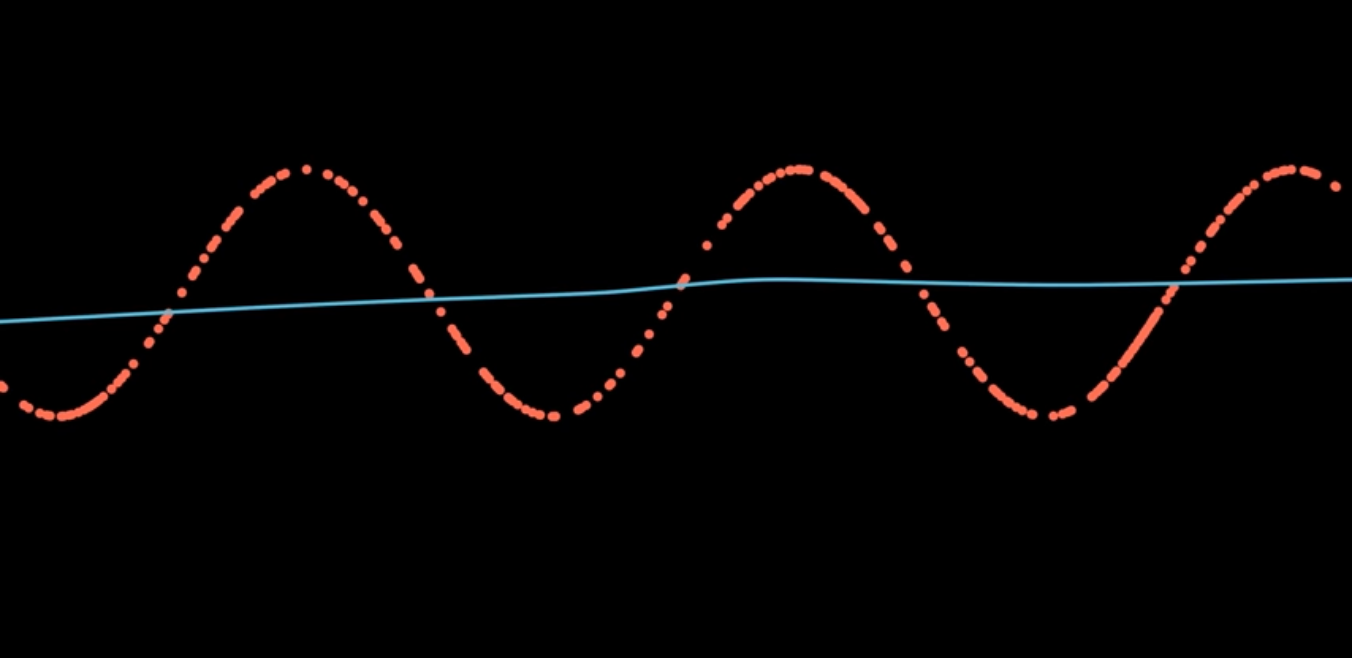
\includegraphics[scale = 0.2]{attachment/chapter_AML/Scc032}
	\caption{Curve fitting inital start}
\end{figure}

After some iteration of weights by tthe process \textit{backpropagation} (General term  \textit{gradient descent}) the \gls{AI_NN} reduces the loss value. 
The \gls{AI_NN} $"$fits$"$ more the target values.
\begin{figure}[H]
	\centering
	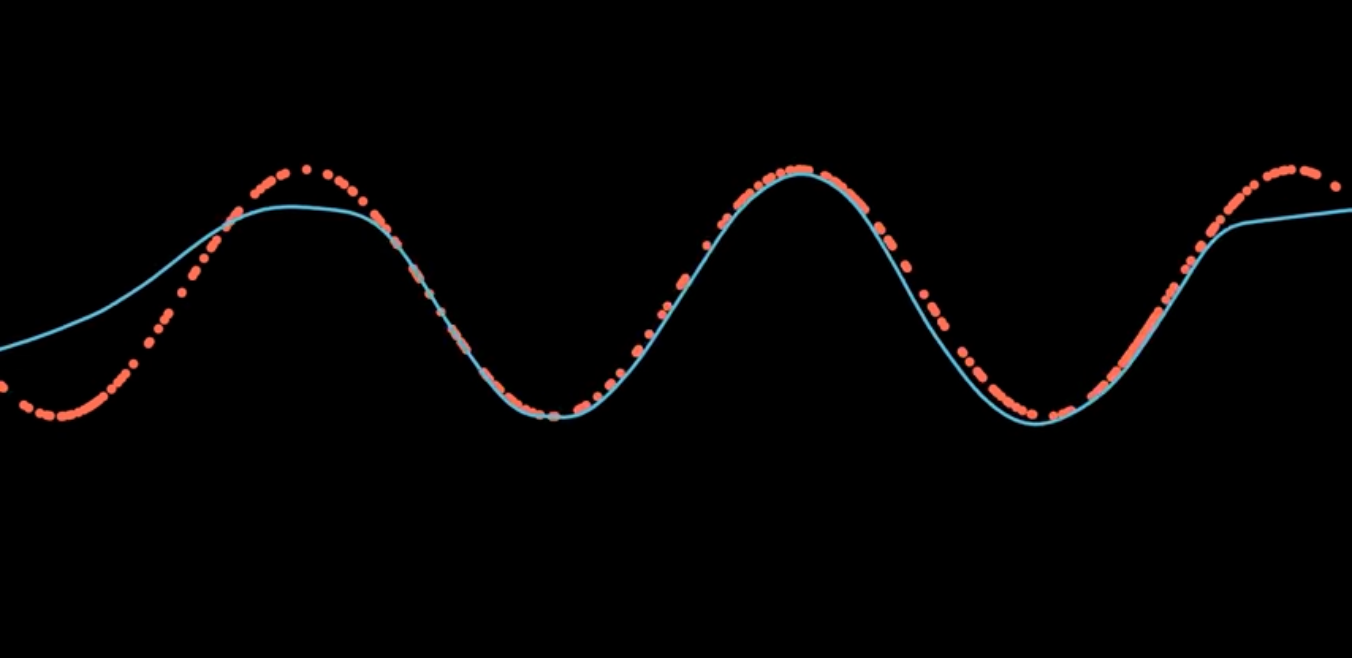
\includegraphics[scale = 0.2]{attachment/chapter_AML/Scc033}
	\caption{Curve fitting after some iteration}
\end{figure}

This process is generalisable and therefore not specific to any function, this is derived from the Universal approximation theorem.
\begin{figure}[H]
	\centering
	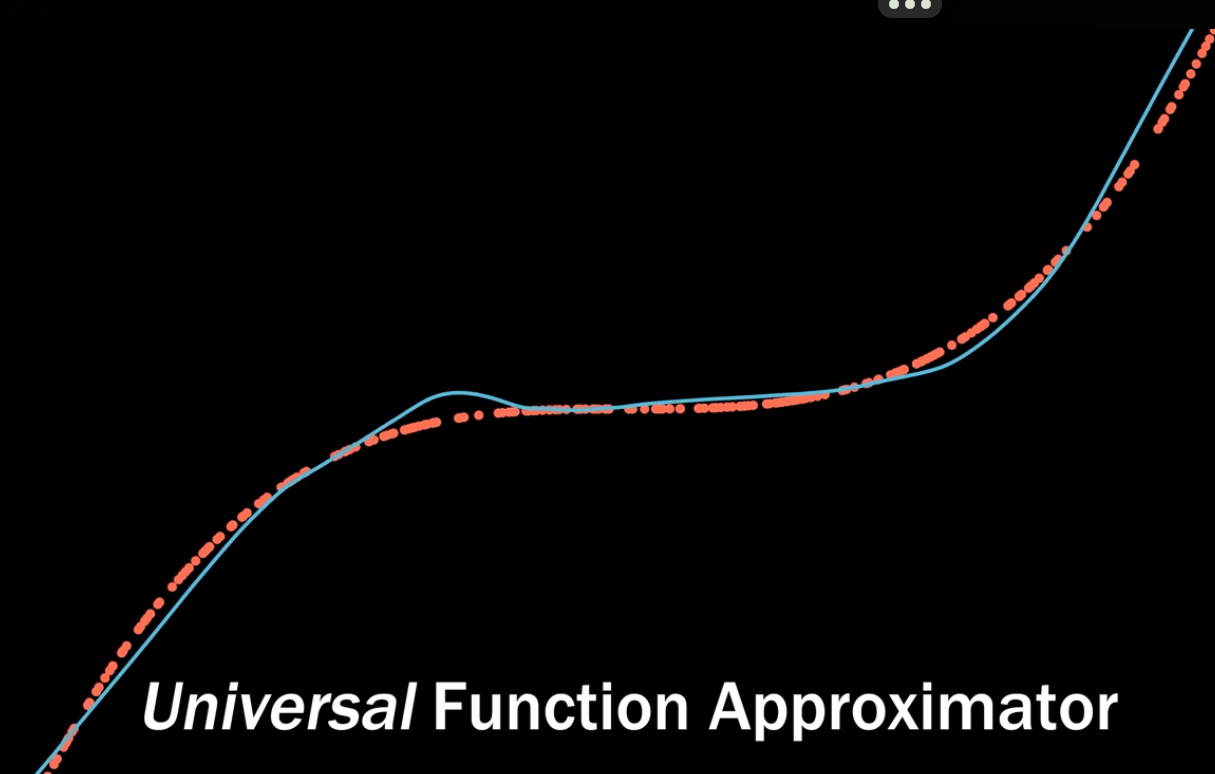
\includegraphics[scale = 0.2]{attachment/chapter_AML/Scc034}
	\caption{A Neural Net as universal function approximator $f(x) \approx NN(x)$}
\end{figure}
	


\subsection{Gradient Descent}
\subsubsection{Optimization Using Gradient Descent}
We now consider the problem of solving for the \textit{minimum} of a real-values function
\begin{align}
	\min_{x} f(x).
\end{align}
We assume
\begin{itemize}
	\item $f:\R^4 \rightarrow R$ captures the machine learning problem at hand,
	\item $f$ is differentiable,
	\item we are unable to analytically find the solution in closed form.
\end{itemize}
The \textit{gradient descent} takes steps a proportionaly ($\gamma$) to the negative of the gradient of the function $\nabla f$ at the current point $x_0$:
\begin{align}
	\nabla x_1 = x_0 - \gamma ((\nabla f)(x_0))^T.
\end{align}
At the point $x_0$ the function $f(x_0)$ degresses fastes if on moves from $x_0$ in the direction of the negative gradient $- \gamma ((\nabla f)(x_0))^T$ of $f$ at $x_0$. From this follows: For a small \textit{step-size}\footnote{In Azure ML is called \textit{learning-rate}} $\gamma \geq 0$ $f(x_1)\geq f(x_0)$.\\

\paragraph{The Simple Gradient Descent Algorithm}
To find the \underline{local} optimum $f_{x_*}$ we start with a inial guess $x_0$ of the parameter we wish to optimize. Then we iterate according to 

\begin{align}
	\nabla x_{i+1} = x_i - \gamma_i ((\nabla f)(x_i))^T.
\end{align}
For a suitable step-size $\gamma_i$, the sequence $f(x_0)\leq f(x_1) \leq ... $ converges to a \textit{local} minimum.

\paragraph{Graphical Gradient Descent}
Only if the step-size $\gamma$ is a big, that the $f(x_{i+1}$ overshots the local minimum, the functional value $y=f(x_{i})$ converges to the local minimum.

\begin{figure}[H]
	\centering
	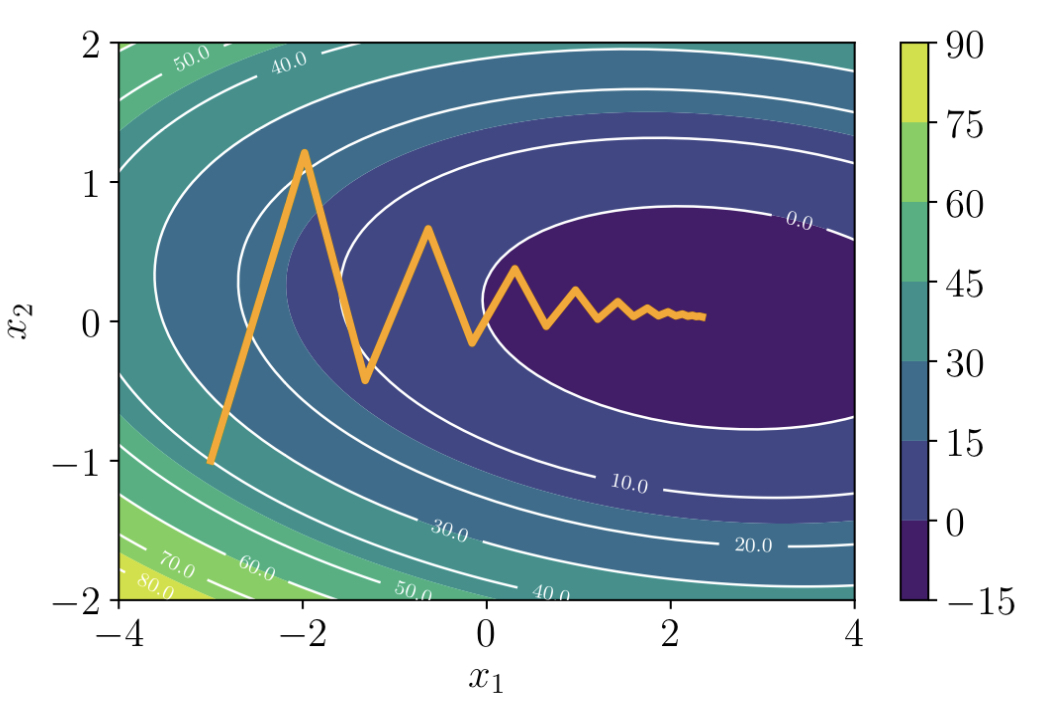
\includegraphics[scale = 0.2]{attachment/chapter_10/Scc053}
	\caption{Graph shows the gradient descent on a two dimensional quadratic surface.}
\end{figure}


The zig-zag of the graph

\begin{figure}[H]
	\centering
	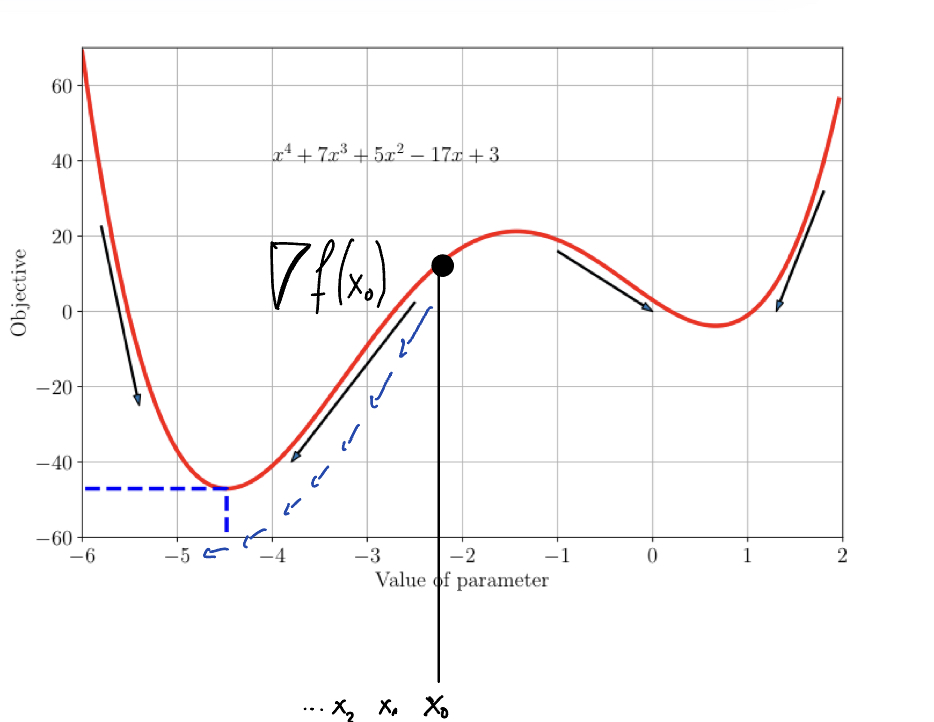
\includegraphics[scale = 0.2]{attachment/chapter_10/Scc052}
	\caption{Example of a one dimentional function. Negative gradient descent is indicated by the arrows.}
\end{figure}

\subsubsection{Solving a Linear Equation System}
\paragraph{In Form Ax=b}
